\documentclass[tikz,border=5pt]{standalone}
\usepackage[T1]{fontenc}
\usepackage{lmodern,amsmath,amssymb}
\usetikzlibrary{arrows.meta,calc,positioning,fit,backgrounds,shapes.geometric,matrix,decorations.pathreplacing,patterns}
\definecolor{ink}{gray}{0.08}
\definecolor{wash}{gray}{0.965}
\definecolor{soft}{gray}{0.45}
\tikzset{box/.style={draw=ink,line width=.65pt,fill=white,align=center,inner sep=4pt,outer sep=0pt,font=\small},flow/.style={draw=ink,line width=.65pt,-{Latex[length=1.8mm,width=1.3mm]},rounded corners=2pt},annotation/.style={font=\scriptsize,text=soft,align=center},groupbox/.style={draw=soft,dashed,line width=.45pt,fill=wash}}
\begin{document}
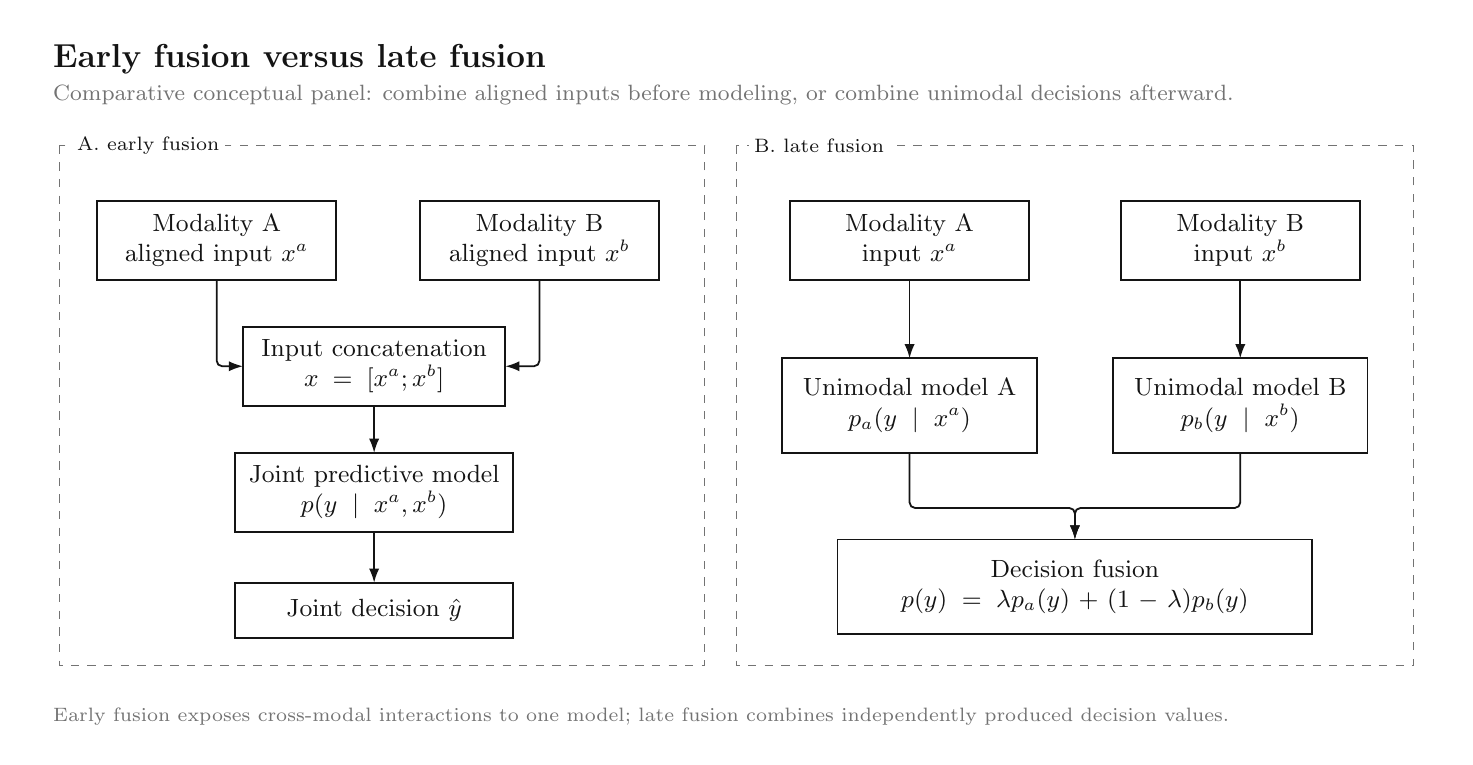
\begin{tikzpicture}[x=1cm,y=-1cm,font=\rmfamily,text=ink]

\path[use as bounding box] (0,0) rectangle (18,9);
\node[anchor=west,font=\large\bfseries] at (.2,.4) {Early fusion versus late fusion};
\node[anchor=west,font=\footnotesize,text=soft] at (.2,.85) {Comparative conceptual panel: combine aligned inputs before modeling, or combine unimodal decisions afterward.};
\begin{pgfonlayer}{background}
\end{pgfonlayer}
\node[box,minimum width=3.0cm,minimum height=1cm,text width=2.75cm] (ea) at (2.4,2.7) {Modality A\\aligned input $x^a$};
\node[box,minimum width=3.0cm,minimum height=1cm,text width=2.75cm] (eb) at (6.5,2.7) {Modality B\\aligned input $x^b$};
\node[box,minimum width=3.3cm,minimum height=1.0cm,text width=3.05cm] (concat) at (4.4,4.3) {Input concatenation\\$x=[x^a;x^b]$};
\node[box,minimum width=3.5cm,minimum height=1.0cm,text width=3.25cm] (joint) at (4.4,5.9) {Joint predictive model\\$p(y\mid x^a,x^b)$};
\node[box,minimum width=3.5cm,minimum height=0.7cm,text width=3.25cm] (epred) at (4.4,7.4) {Joint decision $\hat y$};
\node[box,minimum width=3.0cm,minimum height=1cm,text width=2.75cm] (la) at (11.2,2.7) {Modality A\\input $x^a$};
\node[box,minimum width=3.0cm,minimum height=1cm,text width=2.75cm] (lb) at (15.4,2.7) {Modality B\\input $x^b$};
\node[box,minimum width=3.2cm,minimum height=1.2cm,text width=2.95cm] (amodel) at (11.2,4.8) {Unimodal model A\\$p_a(y\mid x^a)$};
\node[box,minimum width=3.2cm,minimum height=1.2cm,text width=2.95cm] (bmodel) at (15.4,4.8) {Unimodal model B\\$p_b(y\mid x^b)$};
\node[box,minimum width=6.0cm,minimum height=1.2cm,text width=5.75cm] (combine) at (13.3,7.1) {Decision fusion\\$p(y)=\lambda p_a(y)+(1-\lambda)p_b(y)$};
\begin{pgfonlayer}{background}
\draw[flow] (ea.south) -- (2.4,4.3) -- (concat.west);
\draw[flow] (eb.south) -- (6.5,4.3) -- (concat.east);
\draw[flow] (concat.south) -- (joint.north);
\draw[flow] (joint.south) -- (epred.north);
\draw[flow] (la.south) -- (amodel.north);
\draw[flow] (lb.south) -- (bmodel.north);
\draw[flow] (amodel.south) -- (11.2,6.1) -- (13.3,6.1) -- (combine.north);
\draw[flow] (bmodel.south) -- (15.4,6.1) -- (13.3,6.1) -- (combine.north);
\end{pgfonlayer}
\draw[draw=soft,dashed,line width=.45pt] (0.4,1.5) rectangle (8.6,8.1);
\node[anchor=west,font=\scriptsize,fill=white,inner sep=2pt] at (0.55,1.5) {A. early fusion};
\draw[draw=soft,dashed,line width=.45pt] (9.0,1.5) rectangle (17.6,8.1);
\node[anchor=west,font=\scriptsize,fill=white,inner sep=2pt] at (9.15,1.5) {B. late fusion};
\node[anchor=west,align=left,font=\scriptsize,text=soft,text width=17.6cm] at (.2,8.75) {Early fusion exposes cross-modal interactions to one model; late fusion combines independently produced decision values.};
\end{tikzpicture}
\end{document}
